
\section{Dummy-Load}
\label{section:dummy_load_1}
\begin{frame}%STARTCONTENT

\begin{columns}
    \begin{column}{0.48\textwidth}
    \begin{itemize}
  \item \emph{Dummy Load} wird für Abgleicharbeiten und Messungen an Sendern verwendet
  \item Ist ein Lastwiderstand
  \item Sendeleistung wird fast vollständig in Wärme umgesetzt
  \item auch: \emph{Abschlusswiderstand} oder \emph{künstliche Antenne}
  \end{itemize}

    \end{column}
   \begin{column}{0.48\textwidth}
       
\begin{figure}
    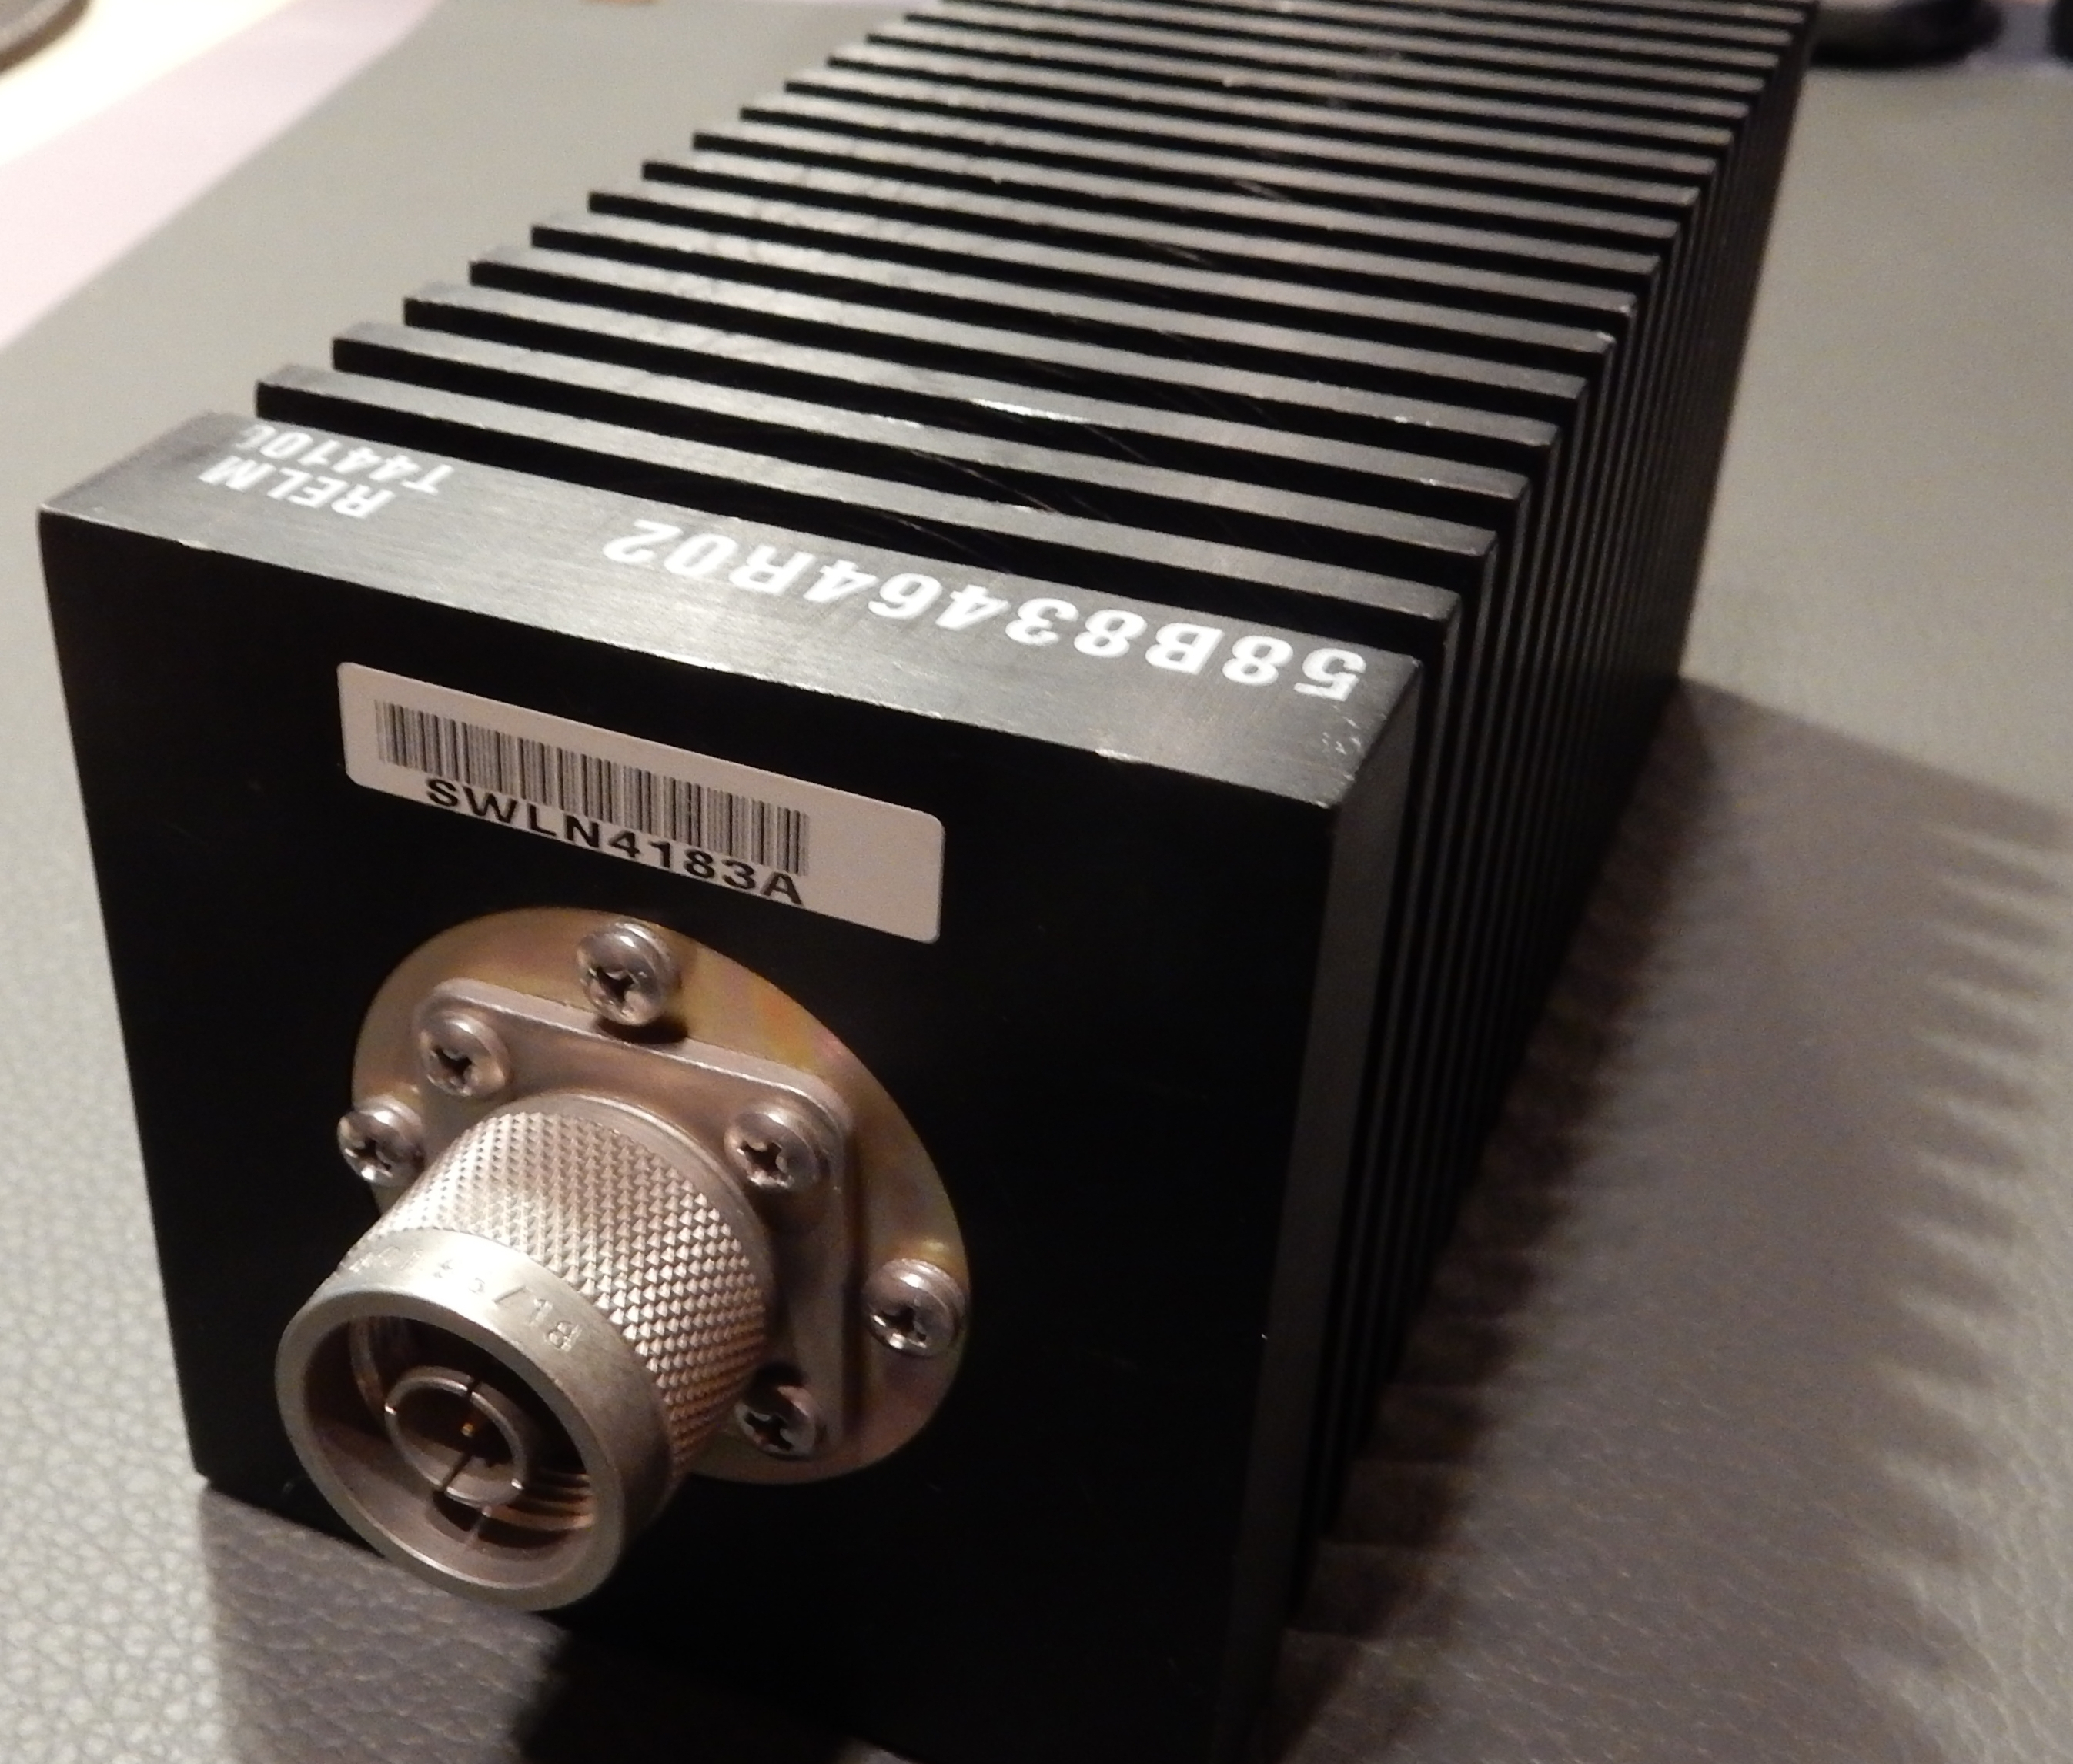
\includegraphics[width=0.85\textwidth]{foto/68}
    \caption{\scriptsize Dummy Load}
    \label{n_antennenanpassung_dummy_load}
\end{figure}

   \end{column}
\end{columns}

\end{frame}

\begin{frame}
\frametitle{Abgleicharbeiten und Messungen}
\begin{itemize}
  \item Immer an möglichst angepasster Antenne oder Dummy Load
  \item Ansonsten kann die Reflektion der Leistung die Endstufe zerstören
  \end{itemize}
\end{frame}

\begin{frame}
\only<1>{
\begin{QQuestion}{VD111}{Was ist bei Abgleicharbeiten und Messungen an Sendern im Hinblick auf die Aussendung zu beachten?}{Das Antennenkabel muss fest angeschlossen sein.}
{Das Sendergehäuse darf nicht geöffnet werden.}
{Es sind geeignete Maßnahmen zu treffen, die ein freies Abstrahlen von Signalen wirkungsvoll verhindern.}
{Es darf nur mit halber Sendeleistung gesendet werden.}
\end{QQuestion}

}
\only<2>{
\begin{QQuestion}{VD111}{Was ist bei Abgleicharbeiten und Messungen an Sendern im Hinblick auf die Aussendung zu beachten?}{Das Antennenkabel muss fest angeschlossen sein.}
{Das Sendergehäuse darf nicht geöffnet werden.}
{\textbf{\textcolor{DARCgreen}{Es sind geeignete Maßnahmen zu treffen, die ein freies Abstrahlen von Signalen wirkungsvoll verhindern.}}}
{Es darf nur mit halber Sendeleistung gesendet werden.}
\end{QQuestion}

}
\end{frame}

\begin{frame}
\only<1>{
\begin{QQuestion}{NJ202}{Wie verhindern Sie beim Abgleichen Ihres selbstgebauten Senders Störungen anderer Funkverbindungen?}{Ich sende nur mit halber Sendeleistung.}
{Ich führe die Abstimmarbeiten auf einer sogenannten ISM-Frequenz aus.}
{Ich verwende einen geeigneten Abschlusswiderstand (Dummy Load).}
{Ich versuche unnötige Modulation zu vermeiden.}
\end{QQuestion}

}
\only<2>{
\begin{QQuestion}{NJ202}{Wie verhindern Sie beim Abgleichen Ihres selbstgebauten Senders Störungen anderer Funkverbindungen?}{Ich sende nur mit halber Sendeleistung.}
{Ich führe die Abstimmarbeiten auf einer sogenannten ISM-Frequenz aus.}
{\textbf{\textcolor{DARCgreen}{Ich verwende einen geeigneten Abschlusswiderstand (Dummy Load).}}}
{Ich versuche unnötige Modulation zu vermeiden.}
\end{QQuestion}

}
\end{frame}

\begin{frame}
\only<1>{
\begin{QQuestion}{NF107}{Warum sollte ein Sender nie ohne angepasste Antenne oder Dummy Load betrieben werden?}{Durch die reflektierte Welle könnte die Senderendstufe beschädigt werden.}
{Durch die fehlende Last wird die Versorgungsspannung hochgeregelt, was zu Überspannungen führen kann. }
{Durch die absorbierte Leistung kann das Netzteil des Senders überlastet werden.  }
{Das Stehwellenmessgerät könnte beschädigt werden.}
\end{QQuestion}

}
\only<2>{
\begin{QQuestion}{NF107}{Warum sollte ein Sender nie ohne angepasste Antenne oder Dummy Load betrieben werden?}{\textbf{\textcolor{DARCgreen}{Durch die reflektierte Welle könnte die Senderendstufe beschädigt werden.}}}
{Durch die fehlende Last wird die Versorgungsspannung hochgeregelt, was zu Überspannungen führen kann. }
{Durch die absorbierte Leistung kann das Netzteil des Senders überlastet werden.  }
{Das Stehwellenmessgerät könnte beschädigt werden.}
\end{QQuestion}

}
\end{frame}

\begin{frame}
\frametitle{Abstimmen}
\begin{itemize}
  \item Aussendungen zum Abstimmen lassen sich nicht vermeiden
  \item Z.B. bei automatischen Anpassgeräten
  \item So kurz wie möglich
  \item Auf freier Frequenz
  \end{itemize}
\end{frame}

\begin{frame}
\only<1>{
\begin{QQuestion}{VD112}{Unter welcher Bedingung ist das Aussenden eines unmodulierten oder ungetasteten Trägers zulässig?}{Sofern es sich um ein digitales Signal handelt}
{Wenn es kurzzeitig erfolgt, z.~B. zum Abstimmen}
{Wenn die Übertragungsbedingungen keine weitreichenden Verbindungen zulassen}
{Sofern die Sendeleistung auf unter \qty{1}{\W} reduziert wird}
\end{QQuestion}

}
\only<2>{
\begin{QQuestion}{VD112}{Unter welcher Bedingung ist das Aussenden eines unmodulierten oder ungetasteten Trägers zulässig?}{Sofern es sich um ein digitales Signal handelt}
{\textbf{\textcolor{DARCgreen}{Wenn es kurzzeitig erfolgt, z.~B. zum Abstimmen}}}
{Wenn die Übertragungsbedingungen keine weitreichenden Verbindungen zulassen}
{Sofern die Sendeleistung auf unter \qty{1}{\W} reduziert wird}
\end{QQuestion}

}
\end{frame}%ENDCONTENT
